\documentclass[10pt]{beamer}

\usepackage{tikz}
\usepackage[labelfont=bf]{caption}
\usepackage{booktabs}
\usepackage{caption}
\usepackage{siunitx}
\usepackage{amsmath}
\usepackage{pgfplots}
\usepackage{pgfplotstable}

\title{Determining the accleration due to gravity via the observation of two simple harmonic oscillators}
\author{Henry Oehlrich}

\begin{document}
\maketitle

\begin{frame}
    \frametitle{Abstract}
\end{frame}

\begin{frame}
    \frametitle{Experiment Setup}
    \begin{minipage}{0.5\textwidth}
        \centering
        \begin{tikzpicture}
            \draw (-2,0) -- (2,0);
            \draw[dashed] (0,0) -- ++(0, -3);
            \draw (0,0) -- ++(-1, -2.6) node [midway, left] {\footnotesize $l$} ++(-0.2, 0) rectangle ++(0.4, -0.4) node [midway] {\footnotesize $m$};
            \draw (0,-0.5) arc [start angle=270, end angle=249, radius=5mm] ++(+0.05,-0.2) node {\footnotesize $\theta$};
        \end{tikzpicture}%
        \vspace{1cm}
        \begin{tabular}{l|l}
            \toprule
            Variable & Description \\
            \midrule
            $L$ & measured length \\
            $m$ & varied mass \\
            $\theta$ & small angle ($<$ \ang{15}) \\
        \end{tabular}
    \end{minipage}%
    \begin{minipage}{0.5\textwidth}
        \centering
        \begin{tabular}{l|l}
            \toprule
            Variable & Description \\
            \midrule
            $m$ & varied mass \\
            $x$ & measured displacement \\
            $x_0$ & initial displacement \\
        \end{tabular}%
        \vspace{1cm}
        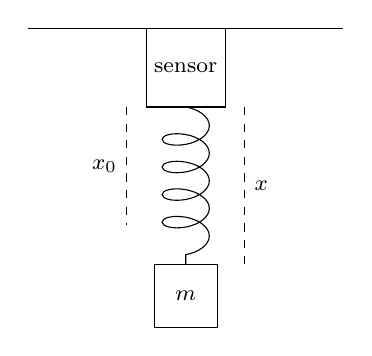
\begin{tikzpicture}
            \draw (-2,0) -- (2,0);
            \draw (-0.5,0) rectangle ++(1, -1) node [midway] {\footnotesize sensor};
            \draw[decorate, decoration={coil, segment length=3.5mm, amplitude=3mm}] (0,-1) -- ++(0, -2);
            \draw (-0.4,-3) rectangle ++(0.8, -0.8) node [midway] {\footnotesize $m$};
            \draw[dashed] (0.75,-1) -- ++(0, -2) node [midway, right] {\footnotesize $x$};
            \draw[dashed] (-0.75,-1) -- ++(0, -1.5) node [midway, left] {\footnotesize $x_0$};
        \end{tikzpicture}
    \end{minipage}
\end{frame}

\begin{frame}
    \frametitle{Materials and Methods}
\end{frame}

\begin{frame} 
    \frametitle{Results} 
\end{frame}

\begin{frame}
    \frametitle{Calculations}
    \begin{minipage}{0.5\textwidth}
        \begin{gather}
            a = -\omega^2x \\
            -\omega = \sqrt{\frac{a}{x}} \\
            \omega = \sqrt{\frac{g}{l}} = \frac{2\pi}{T} \\
            T = 2\pi\sqrt{\frac{l}{g}} \\
        \end{gather}
    \end{minipage}%
    \begin{minipage}
        \begin{gather}
            F = -kx
        \end{gather}
    \end{minipage}
\end{frame}

\begin{frame}
    \frametitle{Pendulum Graphical Relationship}
    \centering
    \begin{tikzpicture}
        \begin{axis}[
                xlabel={$\frac{1}{l}$ (\si{\per\meter})},
                ylabel={$\frac{4\pi^2}{T^2}$ (\si{\newton})},
                tick label style={/pgf/number format/fixed},
                scaled ticks=false,
                width=0.8\textwidth,
                legend pos=south east,
            ]
            \addplot +[only marks,mark size=1.5pt] table
            {pendulum.dat};
            \addplot table [
                y={create col/linear regression={y=y}},
                mark=none,
            ]
            {pendulum.dat};
            \addlegendentry{$\frac{4\pi^2}{T^2} = g\frac{1}{L}$}
            \addlegendentry{$\hat{\frac{4\pi^2}{T^2}} = \pgfmathprintnumber{\pgfplotstableregressiona}(\frac{1}{L})$}
        \end{axis}
    \end{tikzpicture}
\end{frame}

\begin{frame}
    \frametitle{Spring Graphical Relationship}
    \centering
    \begin{tikzpicture}
        \begin{axis}[
                xlabel={$m$ (\si{\meter})},
                ylabel={$kx$ (\si{\newton})},
                tick label style={/pgf/number format/fixed},
                scaled ticks=false,
                width=0.8\textwidth,
                legend pos=south east,
            ]
            \addplot +[only marks,mark size=1.5pt] table
            {spring.dat};
            \addplot table [
                y={create col/linear regression={y=kx}},
                mark=none,
            ]
            {spring.dat};
            \addlegendentry{$mg = kx$}
            \addlegendentry{$\hat{kx} = \pgfmathprintnumber{\pgfplotstableregressiona}{m}$}
        \end{axis}
    \end{tikzpicture}
\end{frame}

\begin{frame}
    \frametitle{Discussion}
\end{frame}

\end{document}
